%\vspace{-0.2in}
\section{Evaluation}
\label{sec:eval}
We evaluate \tool on a variety of problems that can fall under the umbrella of {\it secure prediction}, where one
party (the server) has a machine learning model, and the other party
(the client) has an input. The goal is to compute the output of the
model on client's input, with the guarantee that the server
learns nothing about the input, and the client learns nothing
about the model beyond what is revealed from the output.

To begin, we first implement the benchmarks from Bost et al.~\cite{shafindss}
and \minion~\cite{minionn} (both of which study the same setting),
and show that the performance of the high-level code written in \tool
is comparable to their hand-crafted protocols.
%
Next, we demonstrate the generality and programmability aspects of
\tool by implementing state-of-the-art machine learning models from
Tensorflow~\cite{tensorflow} and \bonsai~\cite{bonsai}. Indeed, we
provide the first 2PC implementation of \bonsai.
%
We
implement a Deep Neural Network (DNN) for CIFAR-10
dataset~\cite{cifar} from \minion~\cite{minionn} and matrix factorization~\cite{valeriaMatrix}
to evaluate partitioning.
%Finally, we evaluate \tool on the task of matrix factorization~\cite{valeriaMatrix}. 

We present the numbers for two network settings, a LAN setting and
a cross-continent WAN setting. The round trip time between the server
and the client machines in the two settings is 1ms and 40ms respectively. Each
machine has an Intel(R) Xeon(R) CPU E5-2673 v3 processor running at
2.40GHz with 28 GBs of RAM. When we compare our execution times with prior protocols, we match our system and network parameters with those of the prior work (as the code for works such as Bost et al. \cite{shafindss} and \minion~\cite{minionn} are not publicly available).
%
%% The  \tool compiler is written in Python and
%% compiles each of our benchmarks in under a second to C++ code that makes calls to the ABY
%% library~\cite{aby}. We use an off-the-shelf solver
%% (SeaHorn~\cite{seahorn}) to check the verification conditions required
%% to prove that the array indices remain in bound. The solver takes less
%% than a minute on our largest benchmark.
Most of our benchmarks
are related to machine learning and we set up (largely standard) notation and describe our benchmarks in \appendixref{benchmarks}.

%\subsection{Benchmarks description}
%\divya{notation can be moved somewhere... } \\

\subsection{Secure prediction}
\paragraph{Standard classifiers.}
%\label{sec:shallow}
We evaluate the three standard classifiers, linear, Na\"{i}ve Bayes, and
decision trees, from~\cite{shafindss} on the following data sets from the UCI
machine learning repository~\cite{uci}:
 the Wisconsin Breast Cancer data set, 
Credit Approval data set, Audiology (Standardized) data set, Nursery
data set, and ECG (electrocardiogram) classification data
from~\cite{barni}.

The results for linear
classification are in Table~\ref{tab:lc}.
The input and the model are both vectors of length $d$. 
The columns ``Prev. time'' and ``Prev. comm'' show the time and the total
network communication reported by Bost et al.~\cite{shafindss} for a
network setting with 40ms
round trip time, which is same as our WAN setting. The total execution
time
of \tool generated code in the LAN and the WAN setting is reported
next, followed by the total communication.
We observe that the \tool code performance matches the hand-crafted protocol of Bost
et al., and the programmer effort in \tool is just 20
lines (last column in the table) of high-level code in the \tool
source language. %\aseem{They write circuits,
 % right?} \nc{Actually, they have a specific protocols for dot product and comparison and also say that their developer effort is minimal as they have to write two function calls to these protocols :).} 
% Our execution time is dominated by the multiplications and
%boolean-ands.
%The number of boolean-and gates (\#And) remains constant for both the
%benchmarks as they reflect the number of gates required for a
%single  comparison, while the number of
%multiplication gates (\#Mul) is the same as the model size $d$.
%% The
%% last column shows the lines of code of \tool program, which is also
%% independent of the model size.

%\setlength\tabcolsep{7pt}
%\begin{table*}
%\begin{tabular}{c|c|c|c|c |c|c|c|c|c|c}
%Dataset & $d$  & Prev. time (s) & Prev. Comm (kb) & LAN (s) & WAN (s) & Comm. (kb)  & \#And & \#Mul & \#Gates & LOC\\
%\hline
%Breast cancer & 30 & 0.3 & 36 & 0.1 & 0.3 & 25 & 95 & 30 & 727 & 20\\
%\hline
%Credit & 47 & 0.3 & 41 & 0.1 & 0.3 & 36 & 95 & 47 & 795 & 20\\
%\hline
%\end{tabular}

\setlength\tabcolsep{2.8pt}
\begin{table}
\footnotesize
\begin{tabular}{|c|c|c|c|c|c|c|c|c|}
\hline
Dataset & $d$  & \thead{Prev \\ time\\ (s)} & \thead{Prev \\ comm\\ (KB)} & \thead{LAN  \\ (s)} & \thead{WAN\\ (s)} & \thead{Comm \\(KB)}  &  \thead{Num \\ gates} & LOC\\
\hline
Breast cancer & 30 & 0.3 & 36 & 0.1 & 0.3 & 25  & 727 & 20\\
\hline
Credit & 47 & 0.3 & 41 & 0.1 & 0.3 & 36  & 795 & 20\\
\hline
\end{tabular}
 \caption{Linear classification results. We compare \tool (LAN, WAN, Comm)
 with~\cite{shafindss} (Prev time, Prev comm).}
 \label{tab:lc} 
\end{table}

%\subsubsection*{Na\"{i}ve Bayes} 


\setlength\tabcolsep{2.5pt}
\begin{table}
\footnotesize
\begin{tabular}{|c|c|c|c|c|c |c|c|c|c|}
\hline
Dataset & $n$ & $F$ & \thead{Prev \\ time\\ (s)} & \thead{Prev \\ comm\\ (KB)} & \thead{LAN  \\ (s)} & \thead{WAN\\ (s)} & \thead{Comm \\(KB)} & \thead{Num \\ gates}  & LOC\\
\hline
Nursery & 5 & 9 & 1.5 & 0.2 & 0.1 & 0.4 & 0.6  & 73k & 50\\
\hline
Audiology & 24 & 70 & 3.9 & 2.0 & 1.5 & 2.9 & 37  & 4219k & 50\\
\hline
\end{tabular}
\caption{Na\"{i}ve Bayes results. We compare \tool (LAN, WAN, Comm)
 with~\cite{shafindss} (Prev time, Prev comm).}
 \label{tab:nb} 
\end{table}


%\subsubsection*{Decision trees}






%\begin{table*}
%\begin{tabular}{|c|c|c|c |c|c|c|c|c|c|c|}
%\hline
%Dataset  & $N$ & \thead{Prev. \\ time\\ (s)} & \thead{Prev. \\ Comm\\ (kb)} & \thead{LAN  \\ (s)} & \thead{WAN\\ (s)} & \thead{Comm. \\(kb)}& \#And & \#Mul &\#Gates & LOC\\
%\hline
%Nursery & 4 & 0.3 & 102 & 0.1 & 0.3 & 32 & 504 & 3 & 3324 & 20\\
%\hline
%ECG &  6 & 0.4 & 102 & 0.1 & 0.4 & 49 & 756 & 5 & 5002 & 20\\
%\hline
%\end{tabular}
% \caption{Decision tree benchmarks. We compare our results (columns 5 , 6, 7) with~\cite{wu} (columns 3 and 4)}
% \label{tab:dt} 
%\end{table*}
\setlength\tabcolsep{3.8pt}

\begin{table}[t]
\footnotesize
\begin{tabular}{|c|c|c|c|c|c|c|c|c|c|}
\hline
Dataset  & $d$ & $N$ & \thead{Prev \\ time\\ (s)} & \thead{Prev \\ comm\\ (KB)} & \thead{LAN  \\ (s)} & \thead{WAN\\ (s)} & \thead{Comm \\(KB)}& \thead{Num \\ gates} & LOC\\
\hline
Nursery & 4 & 4 & 0.3 & 102 & 0.1 & 0.3 & 32 & 3324 & 20\\
\hline
ECG & 4 &  6 & 0.4 & 102 & 0.1 & 0.4 & 49  & 5002 & 20\\
\hline
\end{tabular}
\caption{Decision tree benchmarks.We compare \tool (LAN, WAN, Comm)
 with~\cite{wu} (Prev time, Prev comm).}
 \label{tab:dt} 
\end{table}


%dataset  | size | gates | and | mul | depth | length

%dataset | time | comm | timeL | timeW | comm
%Our decision tree numbers in Table~\ref{tab:dt} further validate
%this claim. 
%We compare with the recent work of Wu et al.~\cite{wu} (columns 3 and 4) who
%describe specialized protocols for trees and forests (that perform
%better than~\cite{shafindss}).
%Similar to Bost et al.~\cite{shafindss}, they also remarks that these
%computations are infeasible with Yao-based 2PC.
%Again, we observe that
%the performance of \tool generated generic 2PC
%code is competitive with specialized protocols. 
The results for Na\"{i}ve Bayes are
in Table~\ref{tab:nb}. As before, $n$ denotes the number of classes and $F$ is the number of features.
%Although, there are no multiplications in these benchmarks, these do
%have a significant number of comparisons (due to array look-ups using
%secret indices) that
%result in many boolean-and gates. %(13k/750k denote 13000/75000). 
As before, we compare with Bost et al.~\cite{shafindss} and observe that \tool generated code
has better performance, despite using a generic 2PC,
as opposed to custom designed protocols developed by Bost et
al. Moreover, they remark that in their setup, generic Yao-based 2PC
did not scale to the smallest of their Na\"{i}ve Bayes classifiers, so
they had to scale down the prediction task, and even then Yao-based \mpc
was 500x slower. Whereas, we show that by using a
cryptographic-cost aware compiler, we can scale generic 2PC to real
prediction tasks, and get performance competitive to or better than the
specialized protocols. Table~\ref{tab:dt} 
compares against the more recent work of~\cite{wu}
on decision trees and further validates this claim.

\paragraph{Deep neural nets.}
We evaluate \tool on the DNNs described in SecureML~\cite{secureml},
Cryptonets~\cite{cryptonets}, and the CNN from \minion~\cite{minionn}. For
comparison, we consider their implementations from
\minion~\cite{minionn}, which outperforms their previous
implementations. Table~\ref{tab:nn} shows the
results\footnote{\minion does not report the network round-trip time nor the bit-length of their inputs (we use $32$-bit inputs).}.
We note that for each of these DNNs, \minion provides a
specialized protocol, while \tool uses a generic 2PC protocol
(auto) generated from high-level code.

The first benchmark  is the DNN described in
SecureML~\cite{secureml} (Figure 10 in~\cite{minionn}).
It has three fully connected layers with square as the activation function.
%This DNN is light-weight as it requires only arithmetic computations
%(additions and multiplications) 
%except for the $\mathsf{argmax}$ at the end of the network.
Next, we implement the DNN described in Cryptonets~\cite{cryptonets} (Figure 11 in~\cite{minionn})
in \tool.
This DNN also uses square as the activation function and has one
convolution (with 5 output channels) and one fully connected layer. 
Finally, we implement CNN from \minion (Figure 12 in~\cite{minionn}), that has
two convolutions (with 16 output channels each) and two fully
connected layers.  In contrast to the previous two DNNs, it uses
ReLU for activation and
has significantly higher number of boolean-and gates.
Note that square activation can be implemented entirely using
arithmetic gates but ReLU requires boolean-and gates.  For a complete
description of these benchmarks and their accuracies, we refer the
reader to the original references. 


%net | minionT | minionC | timeL | timeW | comm | gates | and | mul | length 

%\setlength\tabcolsep{6.5pt}
%\begin{table*}
%\begin{tabular}{c|c|c|c |c|c|c|c|c|c|c}
%DNN  & Prev. time (s) & Prev. Comm (Mb) & LAN (s) & WAN (s) & Comm. (Mb)  & \#And & \#Mul & \#Gates & Model Size & LOC\\
%\hline
%SecureML   &  1.1 & 15.8 & 0.7 & 1.7  & 76   &  2k   & 119k & 366k   & 119k & 78\\
%\hline
%Cryptonets &  1.3 & 47.6 & 0.6 & 1.6  & 70    & 2k    & 108k & 316k & 86k & 88\\
%\hline
%CNN        &  9.4 & 657.5& 5.1 & 11.6 & 501  & 1640k & 667k & 9480k & 35k & 154\\
%\hline
%\end{tabular}
%
% \caption{DNN benchmarks. We compare our results (columns 4 , 5, 6) with~\cite{minionn} (columns 2 and 3)}
% \label{tab:nn} 
%\end{table*}

\setlength\tabcolsep{2.5pt}
\begin{table}
\footnotesize
\begin{tabular}{|c|c|c|c |c|c|c|c|c|}
\hline
DNN  & \thead{Prev \\ time\\ (s)} & \thead{Prev \\ comm\\ (MB)} & \thead{LAN  \\ (s)} & \thead{WAN\\ (s)} & \thead{Comm \\(MB)} & \thead{Num \\ gates} & \thead{Model\\ size} & LOC\\
\hline
SecureML   &  1.1 & 15.8 & 0.7 & 1.7  & 76   &   366k   & 119k & 78\\
\hline
Cryptonets &  1.3 & 47.6 & 0.6 & 1.6  & 70    &  316k & 86k & 88\\
\hline
CNN        &  9.4 & 657.5& 5.1 & 11.6 & 501  & 9480k & 35k & 154\\
\hline
\end{tabular}

 \caption{DNN benchmarks. We compare \tool (LAN, WAN, Comm)
 with~\cite{minionn} (Prev time, Prev comm).}
 \label{tab:nn} 
\end{table}


In Table~\ref{tab:nn}, 
the column ``Model size'' is the number of parameters in the
trained model.
We observe that our performance is competitive with specialized
\minion protocols, for both the LAN and the WAN settings. Further, lines
of \tool source code required is still small. 
%We note that while the \minion implementation is based on the ABY framework, it does not use the framework ``off-the-shelf'' and provide tailor-made optimizations for their applications. %By contrast, \tool focuses on generic
%2PC, exploiting ABY's performant implementation. Optimizations such as those found in \minion are part of our future work.
\minion also reports performance results on a bigger DNN with 7
convolution layers. In \tool, this benchmark requires partitioning and
we discuss it in \sectionref{pipeeval}.

\paragraph{State-of-the-art classifiers.}
Tensorflow~\cite{tensorflow} is a standard machine learning toolkit.
Its introductory tutorial describes two prediction models for handwritten digit recognition
using the MNIST dataset~\cite{mnist}.
Each image in this dataset is a greyscale $28\times 28$ image of
digits 0 to 9.
The first model that the tutorial describes is a softmax regression
that provides an accuracy of 92\%. The classifier evaluates
$ \mathsf{argmax}\ W\matmul x+b$.
Here, $x$ is a 784 length vector obtained from the input image,
 $W$ is a $10\times 784$ matrix, and  $b$ is a $10$ length
vector.
We implement this classifier in \tool and present the results in the
first row of Table~\ref{tab:tf}. 
%We note that a pure boolean circuit for this simple functionality does not fit in the memory of our machines and cannot be evaluated using garbled circuits.


The next classifier in the Tensorflow tutorial is a convolution neural net with two convolutions
(with 32 output channels) and two fully connected layers with ReLU as the activation function.
This DNN is both bigger and more accurate than the DNNs presented in the previous section.
In particular, it has an accuracy of 99.2\%.
Since, we are not aware of any other tools that have used this
model as a benchmark, we only report numbers for \tool.
We observe that this DNN can take a minute per prediction in the WAN
setting and is the largest benchmark that we have evaluated without
partitioning.


% benchmark | size | gates | and | mul | depth  | length | comm | timeL | timeW
\setlength\tabcolsep{2.5pt}
\begin{table}
\footnotesize
\begin{tabular}{|c|c|c|c |c|c|c|c|c|c | c}
\hline
Classifier       & \thead{LAN  \\ (s)} & \thead{WAN \\(s)} & \thead{Comm \\(MB)}  & \thead{Num \\ And} & \thead{Num \\ Mul} & \thead{Num \\ gates} & \thead{Model \\size} & LOC\\
\hline
Regression &  0.1         & 0.7         & 5            & 2k    & 8k    &  35k    & 8k   & 38\\
\hline
CNN        &  30.5        & 60.3        & 2955         & 6082k & 4163k &  42104k & 3226k& 172\\
\hline
\end{tabular}

 \caption{Tensorflow tutorial benchmarks}
 \label{tab:tf} 
\end{table}
\setlength\tabcolsep{3.5pt}
\begin{table}
\footnotesize
\begin{tabular}{|c|c|c|c |c|c|c|c|c|c | c|}
\hline
Dataset       & \thead{LAN \\(s)} & \thead{WAN \\(s)} & \thead{Comm \\ (MB)}  & \thead{Num \\ And} & \thead{Num \\ Mul} & \thead{Num \\ gates} & depth & LOC\\
\hline
Chars4k    &  0.1         & 0.7         & 2            & 18k    & 3k    &  85k     & 1   & 89\\
\hline
USPS       &  0.2         & 0.9         & 4            & 62k    & 2k    &  285k    & 2   & 156\\
\hline
WARD       &  0.3         & 1.1         & 9            & 106k    & 8k    &  506k    & 3   & 283\\
\hline
\end{tabular}

 \caption{Bonsai benchmarks}
 \label{tab:bonsai} 
\end{table}

We next present \bonsai~\cite{bonsai} results on three
standard datasets: character recognition (Chars4k~\cite{campos},
accuracy 74.71\%), text recognition (USPS~\cite{hull}, accuracy
94.4\%), and object categorization (WARD\\~\cite{yang}, accuracy
95.7\%). 
%The \bonsai models are already over integers and no porting from
%floating-point is required.
We implement the trained classifiers in \tool for all the benchmarks
from~\cite{bonsai},
and show the representative results in Table~\ref{tab:bonsai}.
Out of all the benchmarks from~\cite{bonsai}, the dataset WARD
requires the largest model. 
The column ``depth''  shows the depth of the
tree used by \bonsai. The size of \tool 
program grows with the depth of the tree, as the straightforward \tool
implementation requires a loop for each layer of the
tree\footnote{We remark here that our current language does not support functions (which we leave for future work) and with this support, LOC would be lower and independent of depth.}. 

To summarize, by providing first 2PC implementations of
state-of-the-art classifiers, we have demonstrated the expressiveness
of \tool. We discuss scalability next.
%dataset | size | gates | and | mul | depth | length | comm | timeL | timeW


\subsection{Secure code partitioning}
\label{sec:pipeeval}
%\aseem{Is it worth splitting it into microbenchamrking first, which is
 % Fig. 11, and then comparison with others? Right now, Fig. 11 text
 % just comes at the end, should be highlight it in a paragraph or
 % something?}
The largest benchmark of \minion~\cite{minionn} is a DNN for CIFAR-10
dataset~\cite{cifar}. 
The classifier's task is to categorize colored ($32\times 32$) images
into 10 classes. A secure evaluation of this DNN needs more memory
than what is available
on our machines. Therefore, we use partitioning and divide the
computation into seven stages. 
The first step does a convolution with 64 output channels and a ReLU
activation. The next four stages together perform a convolution that
involves multiplying a $64\times 576$ matrix with a 
$576\times 1024$ matrix. The sixth stage performs a ReLU and a
convolution. The final stage has four convolutions, five ReLUs, and a
fully connected layer. The total number of lines of \tool code for
this benchmark is 336 lines.

\setlength\tabcolsep{6pt}
\begin{table}
\footnotesize
\begin{tabular}{|c|c|c|c |c|c|c|}
\hline
           &  LAN (s) & WAN (s) & \thead{Comm \\ (MB)}  & \thead{Num \\ And} & \thead{Num \\ Mul} & \thead{Num \\ gates} \\
\hline
Total      &  265.6       & 647.5        & 40683       & 21m    & 61m    &  337m  \\
\hline
Stage 6    &  55.2        & 122.6        & 6744        & 12m    & 10m   &  98m  \\
\hline
\end{tabular}

 \caption{Partitioning results for CIFAR-10. \minion takes 544 seconds and communicates 9272 Mb.}
 \label{tab:cifar} 
\end{table}

\begin{table}[t]
\footnotesize
\begin{tabular}{|c|c|c|c |c|c| c|}
\hline
  Stage         &  LAN (s) & WAN (s) & \thead{Comm \\ (MB)}  & depth & \thead{Num \\ gates} & LOC\\
\hline
1    &  175       & 662        & 29816       & 16370    & 33m    & 500  \\
\hline
2    &  193        & 1095        & 31945        & 30916    & 37m & 516 \\
\hline
3    &  178        & 627        & 29810        & 16369    & 32m  & 478  \\
\hline
Total    &  546      & 2384        & 91571        & --    & 102m & 1494 \\
\hline
\end{tabular}

 \caption{Partitioning results for matrix factorization. The time reported by~\cite{valeriaMatrix} for this computation is 10440 seconds.}
 \label{tab:factor} 
\end{table}
Table~\ref{tab:cifar} shows the end-to-end numbers as
well as the numbers for the sixth stage, which is the heaviest. 
The number of gates are in millions, hence the suffix `m' in the last
three columns.
%For this DNN, the specialized \minion protocol takes 544 seconds and
%communicates 9272 Mb.
As with Table~\ref{tab:nn}, \tool generated generic 2PC protocol is
competitive with \minion here as well. Therefore,
we believe that with partitioning, \tool can scale to large
computations while maintaining performance
competitive with existing specialized protocols. In particular, for a
large enough DNN, \minion could run
out of memory but an appropriately partitioned \tool implementation would still
succeed.

\paragraph{Scalability.}  To
illustrate the scalability of partitioning, we evaluate a
sequence of DNNs with and without partitioning
(where every layer of each DNN is a separate stage) in~\figureref{partitioning}.
For DNNs with up to 4 (hidden) layers, the performance is almost idential and the lines overlap, thereby
illustrating that partitioning did not cause any noticeable performance overheads.
Memory issues start showing up in the non-partitioned implementation with the 5 layer DNN and it is slower.
Performance degrades rapidly thereafter and
DNNs with 6 or more layers fail to execute (terminate with a ``bus error").
However, the partitioned implementation scales well to even these large DNNs.

\begin{figure}
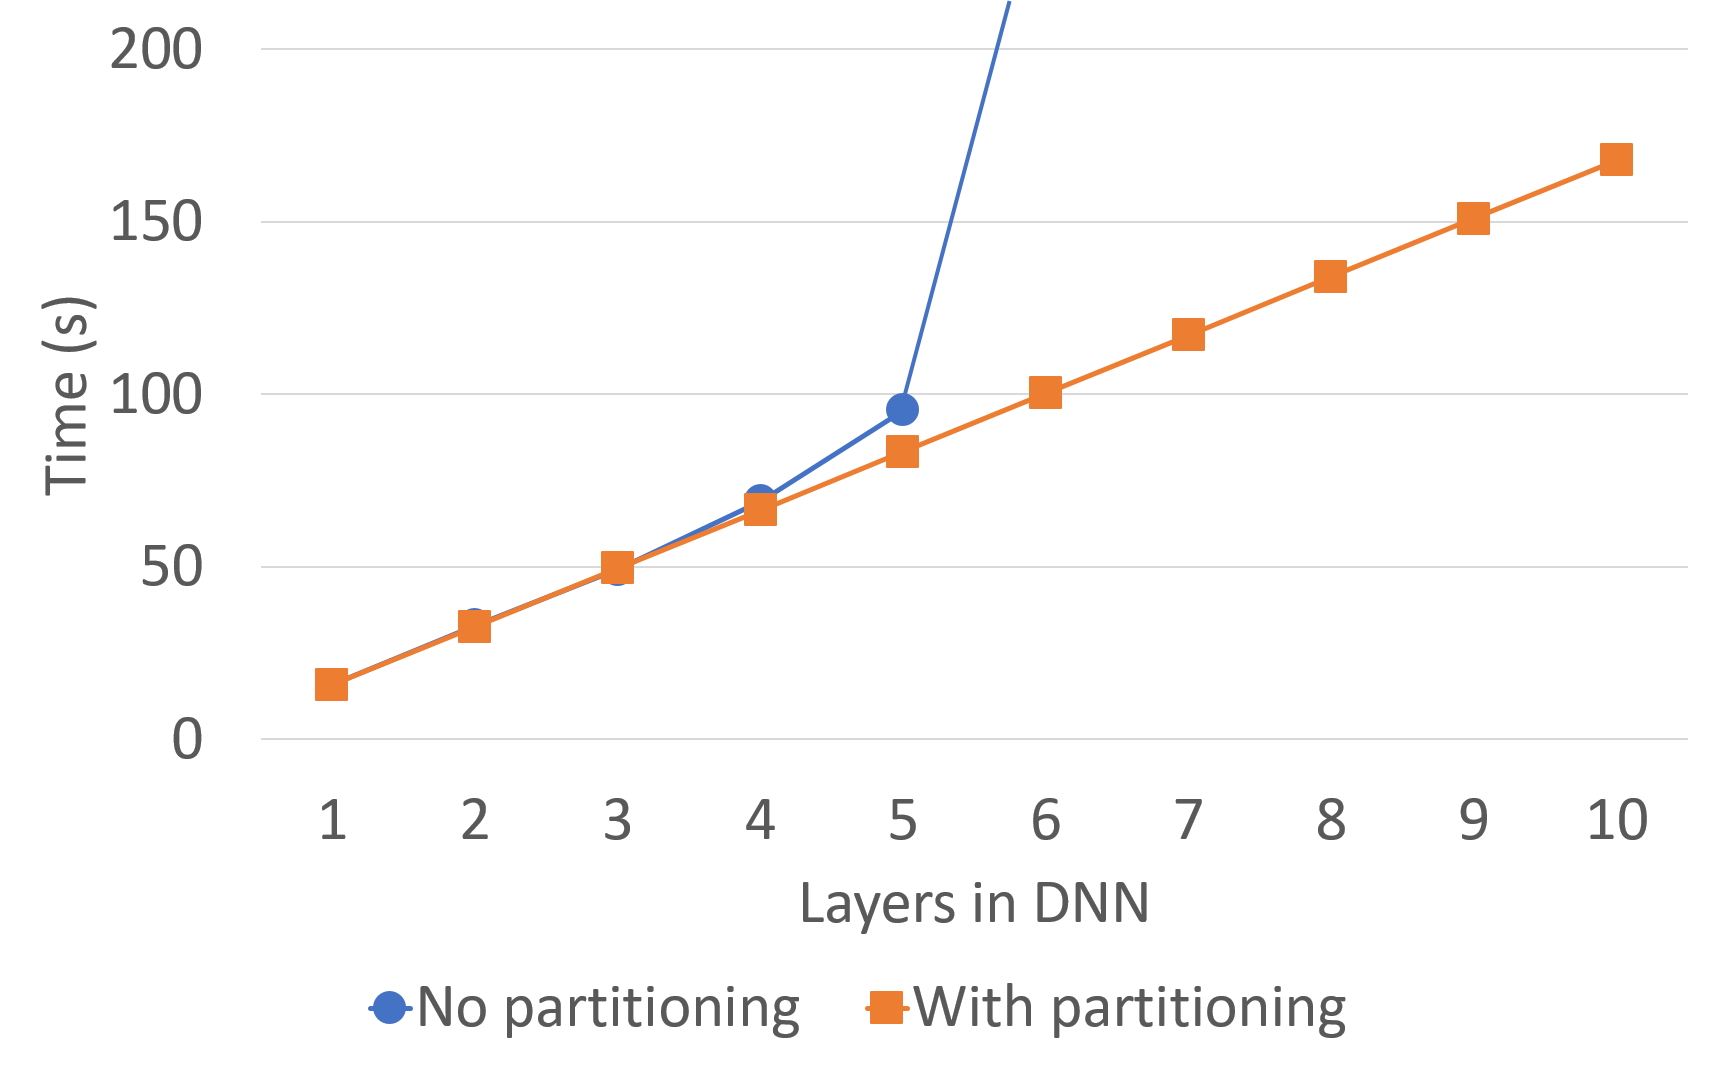
\includegraphics[width=8cm]{partitioning.png}
\caption{Comparison of \tool code with and without partitioning. x-axis denotes the number of layers of the DNN, while y-axis denotes time in seconds for the secure protocol.}
\label{fig:partitioning}
\end{figure}

\subsection{Matrix factorization}
\tool is not tied to secure prediction and can express more general computations.
To demonstrate this expressiveness, we  implement secure matrix factorization~\cite{valeriaMatrix}. Abstractly, given a sparse matrix $\mathcal{M}$ of dimensions
$n\times m$ and $M$ non-zero entries, the goal is to generate a matrix $U$ of dimension $n\times d$ and a matrix
$V$ of dimension $d\times m$ such that $\mathcal{M}\approx UV$. This operator is useful in recommender systems.
In particular, Nikolaenko et al.~\cite{valeriaMatrix} shows how to implement a movie recommender system which does not require users to reveal their data in the clear, i.e., the ratings the users have assigned to movies are kept secret. The implementation is a two party computation of an iterative algorithm for matrix factorization (Algorithm~1 in~\cite{valeriaMatrix}).
This algorithm is based on gradient descent and iteratively converges to a local minima.
We implement this algorithm in \tool.
  
To ensure that the algorithm converges to the right local minima, Nikolaenko et al. require
36 bits of precision. Since ABY supports either 32-bit or 64-bit integers, our \tool implementation
manipulates 64-bit variables. For the matrix $\mathcal{M}$ of  user data, Nikolaenko et al. consider $n=940$ users, $m=40$ most popular movies, and $M=14683$ ratings from the MovieLens dataset. The time reported in~\cite{valeriaMatrix}
for one iteration is 2.9 hours\footnote{~\cite{valeriaMatrix} does not report the network round-trip time.}. This computation is large enough that we partition each iteration
into three stages. The first stage involves a Batcher~\cite{Batcher} sorting network followed by a linear pass.
The second stage involves sorting and gradient computations and is the heaviest stage.
The third  stage is similar to the first stage. The results are presented in Table~\ref{tab:factor}. These circuits have a large depth (column ``depth"); the circuits for secure prediction had depth below 100.


We observe that in the LAN setting, we are about 19 times faster than~\cite{valeriaMatrix} and in the WAN
setting we are about 4 times faster. The main source of these significant speedups is that, unlike~\cite{valeriaMatrix}, \tool does not need to convert the functionality into boolean circuits. 
However, this benchmark requires more lines of code than the previous benchmarks
because of  Batcher's sort (450 lines of \tool code in each stage).
However, the current programmer effort seems miniscule compared to the mammoth implementation effort
put in by Nikolaenko et al. (Section 5 of ~\cite{valeriaMatrix}) to scale a boolean circuits based
backend to this benchmark.

\subsection{Subsequent Work}
Subsequent to our work, Juvekar et al.~\cite{gazelle}  have
presented {\sc Gazelle}, a specialized protocol for DNNs.
{\sc Gazelle} use a lattice-based packed additively homomorphic
encryption scheme (PAHE) for arithmetic computations and garbled
circuits for boolean computations. {\sc Gazelle} can evaluate the CNN benchmark of
Table~\ref{tab:nn} in 0.8 seconds, as opposed to
5.1 seconds taken by \tool with the ABY backend. Such advances in
cryptographic backends are orthogonal to our contributions. In
particular, once {\sc Gazelle} is available, we could add it as another
cryptographic backend to \tool. Furthermore, the authors of Gazelle remark:
``A final, very interesting and ambitious line
of work would be to build a compiler that allows us to easily
express arbitrary computations and automatically factor the
computation into PAHE and two-party primitives'' -- the exact problem
that \tool solves.


%stage | time | comm | gates | mul | add | depth
